\documentclass[
  11pt,
  letterpaper,
   addpoints,
   answers
  ]{exam}

\usepackage{../exercise-preamble}

\begin{document}

\noindent
\begin{minipage}{0.47\textwidth}

\includegraphics[width=\textwidth]{../fcfm_die}
\end{minipage}
\begin{minipage}{0.53\textwidth}
\begin{center} 
\large\textbf{Electromagnetismo Aplicado} (EL3103-1) \\
\large\textbf{Clase auxiliar 2} \\
\normalsize Prof.~Benjamin Jacard H.\\
\normalsize Prof.~Aux.~Erik Saez A.
\end{center}
\end{minipage}

\vspace{0.5cm}
\noindent
\vspace{.85cm}

\begin{questions}
    %%%%%%%%%%%%%%%%%%%%%%%%%%%%
    \question Sean los siguientes problemas:
    \begin{enumerate}
        \item Usa la ley de Gauss para encontrar el campo eléctrico dentro de una esfera sólida uniformemente cargada (densidad de carga \( \rho \)).
        \item Dos esferas, cada una de radio \( R \) y con densidades de carga volumétrica uniformes \( +\rho \) y \( -\rho \), respectivamente, están colocadas de manera que se solapan parcialmente. Llama al vector desde el centro positivo al centro negativo \( d \). Muestra que el campo en la región de solapamiento es constante y encuentra su valor.
        \begin{center}
            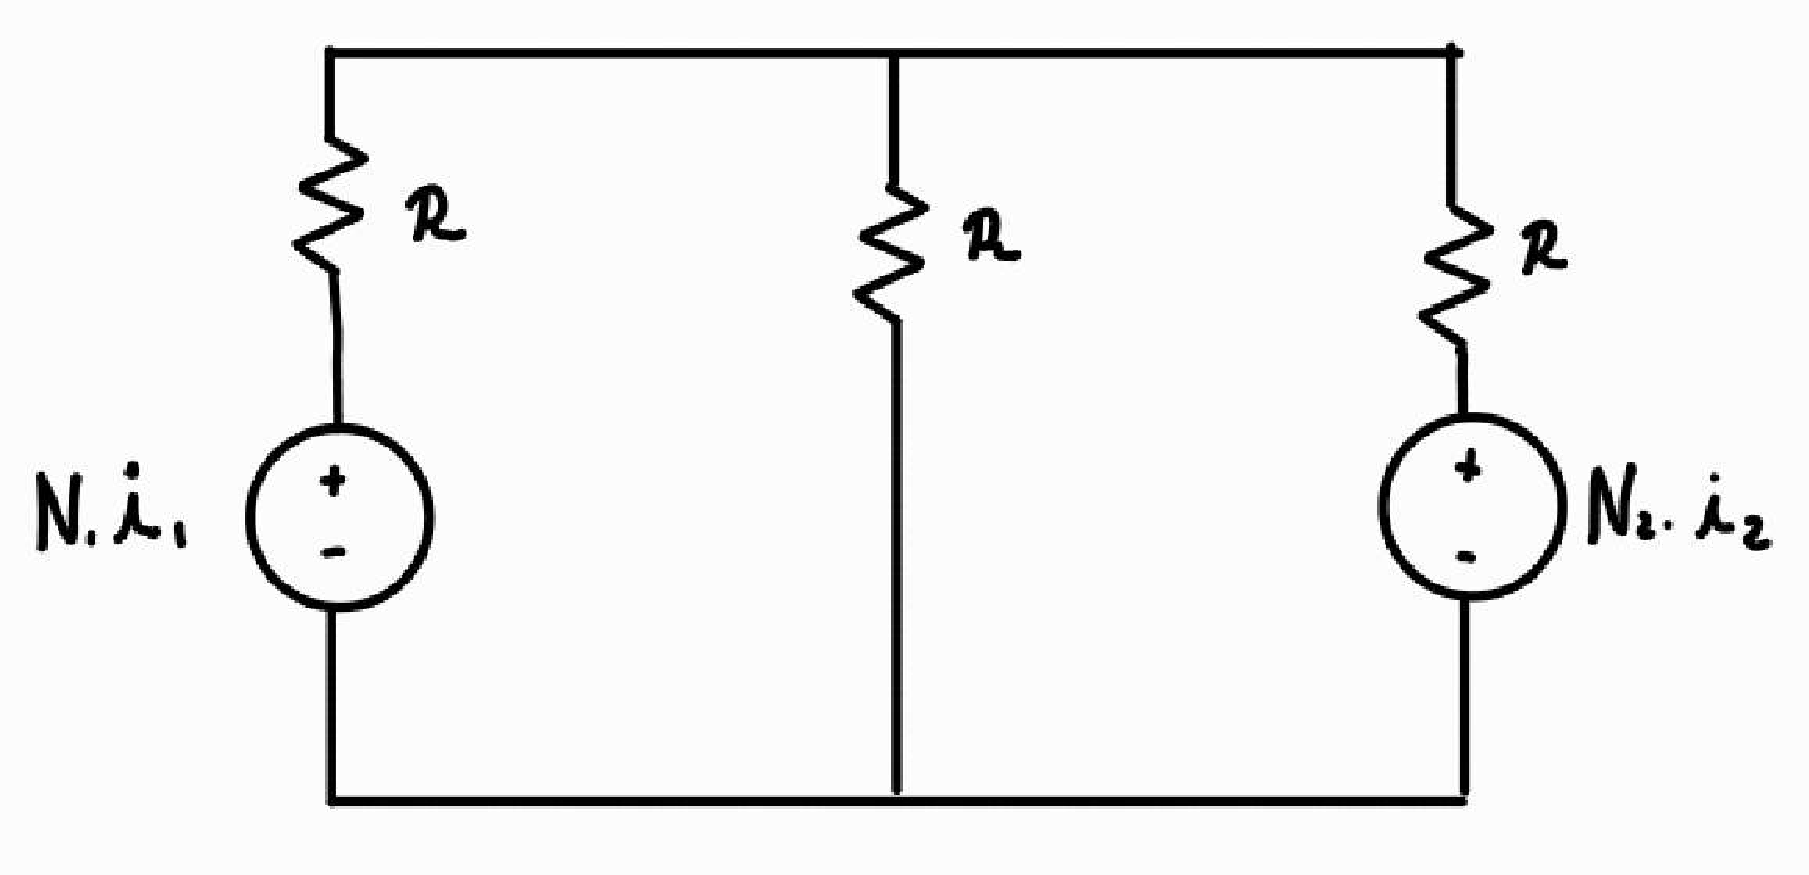
\includegraphics[width=0.25\textwidth]{Auxiliar_2_2}
            \captionof{figure}{Esquema del problema}
        \end{center}
    \end{enumerate}
    %%%%%%%%%%%%%%%%%%%%%%%%%%%%
    \begin{solution}
        La resolucion viene dada por:
        \begin{enumerate}
            \item Se busca obtener el campo eléctrico dentro de una esfera sólida uniformemente cargada, para ello se debe utilizar la ley de Gauss, la cual se puede expresar de la siguiente manera:
            \begin{equation}
                \oint \Vec{E} \cdot \Vec{ds} = \frac{Q_{encerrada}}{\epsilon_{0}}
            \end{equation}
            Dado que se tiene una esfera sólida, se puede considerar una superficie gaussiana esférica, por lo que se tiene que:
            \begin{align}
                \oint \Vec{E} \cdot \Vec{ds} &= \frac{Q_{encerrada}}{\epsilon_{0}}\\
                E \cdot 4\pi r^{2} &= \frac{1}{\epsilon_{0}} \int \rho \cdot dV\\
                E \cdot 4\pi r^{2} &= \frac{1}{\epsilon_{0}} \int \rho \cdot \frac{4}{3}\pi r^{3} \cdot dr\\
                E &= \frac{1}{3\epsilon_{0}} \rho r \hat{r}
            \end{align}
            Es importante considerar que E puede ser sacado de la integral debido a que es constante radialmente, y que dado que estamos dentro de la esfera luego la integral de volumen sera sobre un r y no un R.
            \item Se busca obtener que el campo electrico en la region de solapamiento es constante, para ello recordamos el campo electrico obtenido con anterioridad:
            \begin{equation}
                E = \frac{1}{3\epsilon_{0}} \rho r \hat{r}
            \end{equation}
            Luego es posible realizar lo siguiente:
            \begin{center}
            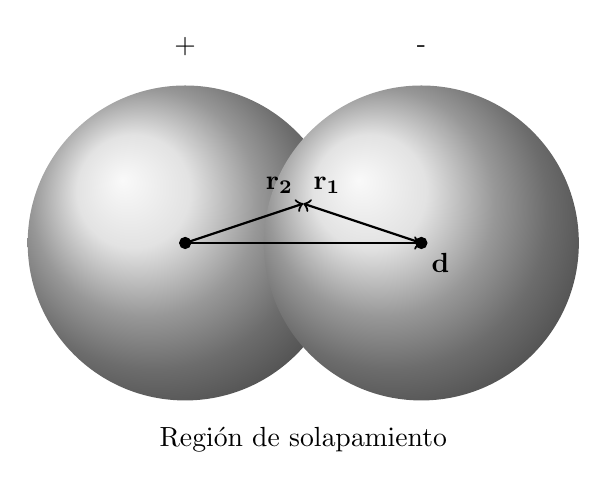
\begin{tikzpicture}
                % Dibuja las esferas
                \shade[ball color=gray!30] (0,0) circle(2);
                \shade[ball color=gray!30] (3,0) circle(2);
                
                % Dibuja los vectores r1 y r2
                \draw[->, thick] (0,0) -- (1.5, 0.5) node[above right] {$\mathbf{r_1}$};
                \draw[->, thick] (3,0) -- (1.5, 0.5) node[above left] {$\mathbf{r_2}$};
                
                % Etiquetas
                \node at (0, 2.5) {+};
                \node at (3, 2.5) {-};
                \node at (1.5, -2.5) {Región de solapamiento};
                
                % Dibuja el vector d
                \draw[->, thick] (0,0) -- (3,0) node[below right] {$\mathbf{d}$};
                
                % Opcional: dibujar los centros de las esferas
                \filldraw[black] (0,0) circle (2pt);
                \filldraw[black] (3,0) circle (2pt);
                
            \end{tikzpicture}     
        \end{center}       
            Debido a la superposicion, luego tendremos que en tal punto el campo electrico sera la suma de ambos campos electricos, por lo que se tendra que:
            \begin{align}
                \sum E_{n} &= E_{1} + E_{2}\\
                           &= \frac{1}{3\epsilon_{0}} \rho r_{1} \hat{r_{1}} - \frac{1}{3\epsilon_{0}} \rho r_{2} \hat{r_{2}}\\
                           &= \frac{1}{3\epsilon_{0}} \rho (r_{1} - r_{2}) \hat{r}
            \end{align}
            Dado lo anterior tenemos que la resta de  \( r_{1} - r_{2} \) sera igual a \( d \), por lo que se tendra que:
            \begin{equation}
                \sum E_{n} = \frac{1}{3\epsilon_{0}} \rho d \hat{r}
            \end{equation}
            Lo cual demuestra que el campo electrico en la region de solapamiento es constante y su valor es \( \frac{1}{3\epsilon_{0}} \rho d \hat{r} \).
        \end{enumerate}
    \end{solution}
    %%%%%%%%%%%%%%%%%%%%%%%%%%%%
    \question  Considere un condensador cuyo dieléctrico de permitividad $\epsilon$ está limitado por dos esferas concéntricas de radios a y b y dos conos equipotenciales de semiángulos $\theta_{1}$ y $\theta_{2}$ como se indica en la figura. Se busca obtener lo siguiente:
    \begin{enumerate}
        \item Obtenga el potencial $\phi_{e}(r,\theta,\phi)$ 
        \item Campo eléctrico \textbf{E}
        \item Capacitancia \textbf{C} a partir de la carga 
        \item Capacitancia \textbf{C} a partir de la energía 
    \end{enumerate}
    \begin{center}
        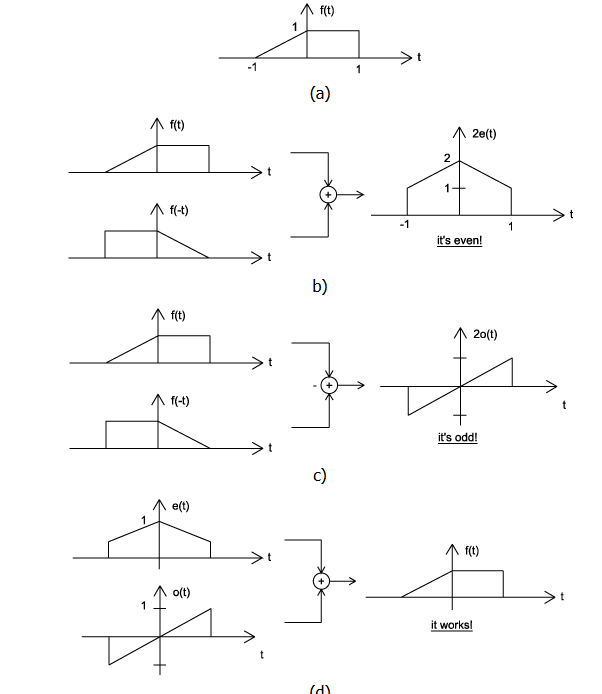
\includegraphics[width=0.4\textwidth]{Auxiliar_2_3}
        \captionof{figure}{Esquema del problema}
    \end{center}
    %%%%%%%%%%%%%%%%%%%%%%%%%%%%
    \begin{solution}
         La resolución viene dada por:
    \begin{enumerate}
        \item Se busca obtener el potencial escalar eléctrico $\phi_{e}$, para la figura en rotación. Se observa que es de conveniencia el utilizar coordenadas esféricas, además que el potencial magnético dependerá solo de $\theta$ y también se considera que no existe densidad de carga libre en el dielectrico (\textit{Si existe en las placas, pero no tenemos informacion acerca de su densidad}), por tanto podemos utilizar la ecuación de Laplace tal que:
        \begin{equation}
            \begin{aligned}
                \nabla^{2}\psi (r,\theta,\phi) &= \frac{1}{r^{2}}\frac{d}{dr}\left(r^{2}\frac{d\psi}{dr}\right) + \frac{1}{r^{2}sin(\theta)}\dfrac{d}{d\theta}\left(sin(\theta) \frac{d\psi}{d\theta}\right) \\
                &\quad + \frac{1}{r^{2}sin^{2}(\theta) }\frac{d^{2}\psi}{d\phi^{2}} = 0
            \end{aligned}
        \end{equation}
        Debido a la dependencia en una sola componente para el potencial tenemos lo siguiente:
        \begin{equation}
            \begin{aligned}
                \nabla^{2}\phi_{e}(\theta) &=  \frac{1}{r^{2}sin(\theta)}\dfrac{d}{d\theta}\left(sin(\theta) \frac{d\phi_{e}}{d\theta}\right) = 0, \\
                sin(\theta) \frac{d\phi_{e}}{d\theta} &= A, \\
                \frac{d\phi_{e}}{d\theta} &= \frac{A}{sin(\theta)}, \\
                \phi_{e}(\theta) &= A\ln\left(\tan( \theta/2) \right) + B.
            \end{aligned}
        \end{equation}
        De esta manera se obtiene la forma general del potencial escalar eléctrico $\phi_{e}$. Luego se deben obtener las ecuaciones de borde para determinar las constantes que caracterizan este sistema. Al ser solo un medio, se simplifica un poco mas el sistema. Para la primera condición:
        \begin{equation}
            \begin{aligned}
                \phi_{e}(\theta = \theta_{1}) &= V_{0}, \\
                V_{0} &= A \cdot \ln\left(\tan(\theta_{1}/2)\right) + B.
            \end{aligned}
        \end{equation}
        Para la segunda condición de borde:
        \begin{equation}
            \begin{aligned}
                \phi_{e}(\theta = \theta_{2}) &= 0, \\
                0 &= A\cdot \ln\left(\tan(\theta_{2}/2)\right) + B.
            \end{aligned}
        \end{equation}
        Luego despejando las constantes obtenemos lo siguiente:
        \begin{equation}
            \begin{aligned}
                A &= \frac{V_{0}}{\ln\left(\frac{\tan(\theta_{1}/2)}{\tan(\theta_{2}/2)}\right)}, \\
                B &=  -\frac{V_{0}}{\ln\left(\frac{\tan(\theta_{1}/2)}{\tan(\theta_{2}/2)}\right)} \cdot \ln\left(\tan(\theta_{2}/2)\right).
            \end{aligned}
        \end{equation}
        
        Obteniendo la forma particular del potencial escalar eléctrico:
        
        \begin{equation}
            \begin{aligned}
                \phi_{e}(\theta) &= A\cdot \ln\left(\tan(\theta/2)\right) + B \\
                &= \frac{V_{0}}{\ln\left(\frac{\tan(\theta_{1}/2)}{\tan(\theta_{2}/2)}\right)} \cdot \ln\left(\tan(\theta/2)\right) \\
                &\quad - \frac{V_{0}}{\ln\left(\frac{\tan(\theta_{1}/2)}{\tan(\theta_{2}/2)}\right)} \cdot \ln\left(\tan(\theta_{2}/2)\right).
            \end{aligned}
        \end{equation}
    \item Se busca obtener el campo eléctrico $\textbf{E}$ el cual se puede obtener de manera directa mediante el campo escalar eléctrico y el hecho de que $\textbf{E}$ es conservativo, por tanto:
    \begin{equation}
        E= - \nabla \phi_{e}(\theta)
    \end{equation}
    Se deberá tener en cuenta que estamos en coordenadas esféricas, por lo que tendremos lo siguiente:
    \begin{equation}
        \nabla \psi = \frac{\partial \psi}{\partial r} \hat{r} + \frac{1}{r} \frac{\partial \psi}{\partial \theta} \hat{\theta} + \frac{1}{r \sin \theta} \frac{\partial \psi}{\partial \phi} \hat{\phi}
    \end{equation}
    Luego reemplazando el potencial escalar obtenido con anterioridad, se tendra:
    \begin{equation}
        \begin{aligned}
            \textbf{E} &= -\frac{1}{r}\frac{d\phi_{e}}{d\theta} \hat{\theta} \\
                       &= \text{\footnotesize$-\frac{1}{r} \frac{d}{d\theta}\left( \frac{V_{0}}{\ln\left(\frac{\tan(\theta_{1}/2)}{\tan(\theta_{2}/2)}\right)} \cdot \ln(\tan(\theta/2)) -\frac{V_{0}}{\ln\left(\frac{\tan(\theta_{1}/2)}{\tan(\theta_{2}/2)}\right)} \cdot \ln(\tan(\theta_{2}/2))\right) \hat{\theta}$} \\
                       &= \frac{-1}{r} \frac{V_{0}}{\ln\left(\frac{\tan(\theta_{1}/2)}{\tan(\theta_{2}/2)}\right)}  \frac{d}{d\theta} \left( \ln(\tan(\theta/2)) \right) \hat{\theta} \\
                       &=\frac{-1}{r} \frac{V_{0}}{\ln\left(\frac{\tan(\theta_{1}/2)}{\tan(\theta_{2}/2)}\right)} \frac{1}{\tan(\theta/2)} \frac{d}{d\theta}\left(\ln(\theta/2)\right)\hat{\theta} \\
                       &= \frac{-1}{2r} \frac{V_{0}}{\ln\left(\frac{\tan(\theta_{1}/2)}{\tan(\theta_{2}/2)}\right)}\frac{\cos(\theta/2)}{\sin(\theta/2)}\cdot \frac{1}{\cos^{2}(\theta/2)}\hat{\theta} \\
                       &=\frac{-1}{r} \frac{V_{0}}{\ln\left(\frac{\tan(\theta_{1}/2)}{\tan(\theta_{2}/2)}\right)}\frac{1}{2\sin(\theta/2)\cos(\theta/2)}\hat{\theta} \\
                       &=\frac{-1}{r} \left(\frac{V_{0}}{\ln\left(\frac{\tan(\theta_{1}/2)}{\tan(\theta_{2}/2)}\right)}\frac{1}{\sin(\theta)}\right)\hat{\theta}
        \end{aligned}
    \end{equation}
    Finalmente, se obtiene el campo eléctrico en base al potencial $\phi_{e}$. Es importante notar que si bien el potencial era una función de $\theta$, el campo eléctrico no dependerá de esta sola componente necesariamente y podrá depender de más. Como es el caso obtenido, el cual dependerá tanto de \textbf{r} como de \textbf{$\theta$} tal que \textbf{E}$(r,\theta)$.
    \item Se busca obtener la capacitancia $C$ en base a la carga. Es importante notar que este término deberá estar expresado en constantes geométricas del material y no en alguna dependencia de una variable (\textit{Puede ser un buen indicador para saber si el ejercicio está bien realizado}).
    \begin{equation}
        C = \frac{Q}{\Delta V}
    \end{equation}
    Sabemos que la diferencia de potencial entre ambas placas corresponderá a $\Delta V = V_{0}$, por lo que $ C = \frac{Q}{V_{0}}$. Utilizando la ley de Gauss tendremos la siguiente relacion:
    \begin{equation}
            \oint \Vec{D} \cdot \Vec{ds} = Q_{encerrada} 
    \end{equation}
    Luego dado que conocemos el valor del desplazamiento eléctrico, se toma una superficie Gaussiana que encierre cualquiera de las placas, eso se resume en considerar que $\vec{ds}=  r\cdot \sin(\theta)(dr) (d\theta)$, dado que es la unica coordenada de interes, y por tanto se tendra que:
    \begin{equation}
        \begin{aligned}
            Q &= -\epsilon \int \frac{-1}{r} \frac{V_{0}}{\ln\left(\frac{\tan(\theta_{1}/2)}{\tan(\theta_{2}/2)}\right)}\frac{1}{\sin(\theta)}(\hat{\theta}) \cdot r\cdot \sin(\theta)(dr) (d\theta)(\hat{\theta}) \\
              &=  \frac{-V_{0}\epsilon}{\ln\left(\frac{\tan(\theta_{1}/2)}{\tan(\theta_{2}/2)}\right)} \int_{0}^{2\pi} \int_{a}^{b} dr d\theta \\
              &=  \frac{V_{0}\epsilon}{\ln\left(\frac{\tan(\theta_{1}/2)}{\tan(\theta_{2}/2)}\right)} \cdot(2\pi)(a-b)
        \end{aligned}
    \end{equation}
    Otra manera de entenderlo, por si se complica entender dicha superficie es lo siguiente:
    \begin{align}
        \oint \Vec{D} \cdot \Vec{ds} &= Q_{encerrada} \\
        \Vec{D} \cdot \Vec{ds} &= \rho_{f} \cdot dV \\
    \end{align}
    Tomando una superficie Gaussiana A, tenemos que:
    \begin{align}
        \Vec{D} \cdot \Vec{ds} &= \rho_{f} dS \\
        D \cdot A &= \rho_{f} A\\
        D &= \rho_{f} \cdot \hat{n}
    \end{align}
    Donde $\rho_{f}$ es la densidad de carga superficial y $\hat{n}$ es el vector normal a la superficie. Finalmente se obtiene la capacitancia en base a la carga, tal que:
    \begin{equation}
        \begin{aligned}
            C &= \frac{Q}{V_{0}} \\
              &= \frac{(a-b)  \cdot 2\pi \cdot \epsilon}{\ln\left(\frac{\tan(\theta_{1}/2)}{\tan(\theta_{2}/2)}\right)}
        \end{aligned}
    \end{equation}
    \item Se busca obtener la capacitancia desde un punto de vista energético. Esto se puede relacionar con la siguiente expresión:
    \begin{equation}
        \frac{1}{2}C V^{2} = \int \frac{1}{2}\epsilon \|E\|^{2} dv
    \end{equation}
    \begin{equation}
        \begin{aligned}
            CV_{0}^{2} &= \epsilon \int \frac{1}{r^{2}}  \frac{V_{0}^{2}}{\ln\left(\frac{\tan(\theta_{1}/2)}{\tan(\theta_{2}/2)}\right)^{2}}\frac{1}{\sin^{2}(\theta)} \cdot r^{2} \cdot \sin(\theta) (d\theta) (d\phi) (dr)
        \end{aligned}
    \end{equation}
    \begin{equation}
        \begin{aligned}
            C &= \frac{\epsilon}{{\ln\left(\frac{\tan(\theta_{1}/2)}{\tan(\theta_{2}/2)}\right)^{2}}} \int_{a}^{b} \int_{0}^{2\pi} \int_{\theta_{1}}^{\theta_{2}}\frac{1}{\sin(\theta)} (d\theta) (d\phi) (dr)
        \end{aligned}
    \end{equation}
    \begin{equation}
        \begin{aligned}
            C &= \frac{\epsilon}{{\ln\left(\frac{\tan(\theta_{1}/2)}{\tan(\theta_{2}/2)}\right)^{2}}} (b-a) \cdot 2\pi \cdot \ln\left(\frac{\tan(\theta_{1}/2)}{\tan(\theta_{2}/2)}\right)
        \end{aligned}
    \end{equation}
    \begin{equation}
        \begin{aligned}
            C &=\frac{(a-b)  \cdot 2\pi \cdot \epsilon}{\ln\left(\frac{\tan(\theta_{1}/2)}{\tan(\theta_{2}/2)}\right)}
        \end{aligned}
    \end{equation}
    Con lo que finalmente se obtiene la capacitancia desde un punto de vista energético, dando así consistencia al problema, dado lo obtenido con anterioridad. 
    \end{enumerate}         
    \end{solution}
    %%%%%%%%%%%%%%%%%%%%%%%%%%%
    \question  Dos barras macizas de sección rectangular se alinean tal que las caras próximas entre las barras son planas y oblicuas, formando los diferentes ángulos mostrados en la Figura y con una diferencia de potencial magnético escalar IN. Las caras oblicuas son de longitud L y ancho b. El espacio entre las caras oblicuas se llena con dos materiales de constantes magnéticas $\mu_{1}$ y $\mu_{2}$ se debe obtener lo siguiente:
    \begin{enumerate}
        \item Obtenga una expresión explícita para el campo magnético escalar $\phi_{m}$ así como para $H_{i}$ en los diferentes medios 
        \item  Obtenga el valor de la inductancia (Considere que la corriente $I_{0}$ es producida por un devanado tal que pueda utilizar la expresión conocida)
        \item Obtenga la energía magnética total del sistema 
    \end{enumerate}
    \begin{center}
        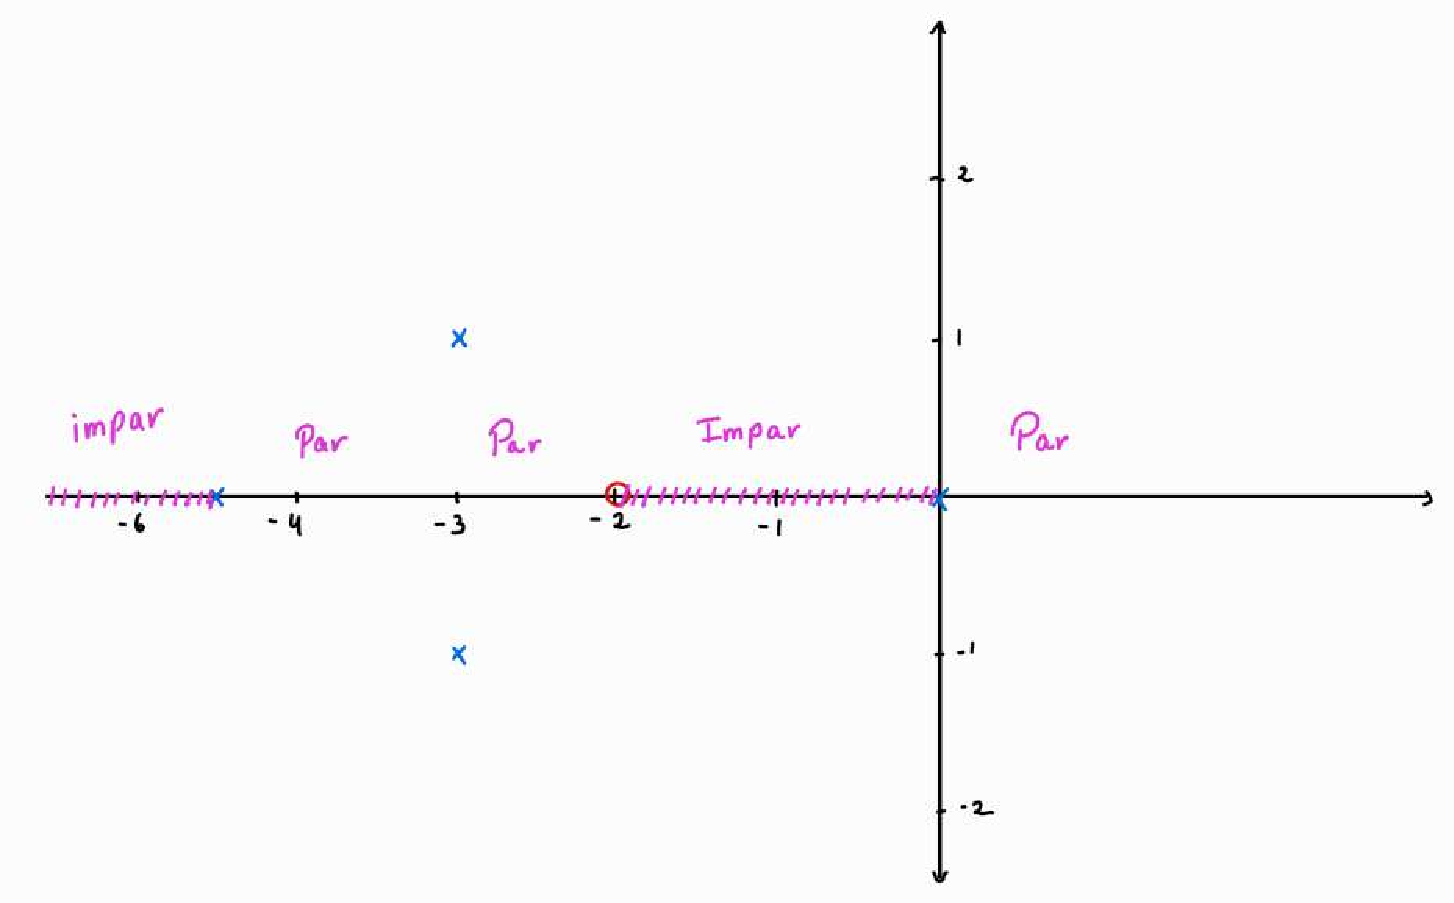
\includegraphics[width=0.7\textwidth]{Auxiliar_2_1}
        \captionof{figure}{Esquema del problema}
    \end{center}
    %%%%%%%%%%%%%%%%%%%%%%%%%%%
    \begin{solution}
        \begin{enumerate}
            \item Dado el esquema se considerará una equivalencia a una \textbf{fuente de voltaje desde el punto de vista magnético}, lo que permitirá generar así un potencial escalar magnético entre ambos medios y por tanto el definir un $H_{1}$ y $H_{2}$, es decir:
            \begin{align}
                H_{i}= -\nabla \phi_{mi}
            \end{align}
            De esta manera se debe encontrar la expresión general para el potencial magnético. Además, se debe analizar qué dirección presentará este y qué tipo de coordenadas es el adecuado para trabajar. Dada la geometría lo más recomendado a utilizar es coordenadas cilíndricas y que el potencial dependa solo de $\phi_{mi}(r,\theta,z) = \phi_{mi}(\theta)$, luego se tendrá:
            \begin{align}
                \nabla^{2}\phi_{mi}(\theta) = \frac{1}{r^{2}}\left(\frac{\partial^{2}\phi_{mi}}{\partial\theta^{2}}\right)= 0
            \end{align}
            Luego encontramos una expresión general para dicho campo magnético, tal que:
            \begin{align}
                \frac{1}{r^{2}} \left(\frac{\partial^{2}\phi_{mi}}{\partial\theta^{2}}\right) &= 0\\
                \frac{\partial^{2}\phi_{mi}}{\partial\theta^{2}} &=0\\
                \frac{\partial^{2}\phi_{mi}}{\partial\theta^{2}} &=0\\
                \frac{\partial \phi_{mi}}{\partial \theta} &= A\\
                \phi_{mi}(\theta) &= A\theta + B 
            \end{align}
            Se debe considerar los dos medios que presentes, por tanto:
            \begin{align}
                \phi_{m1}(\theta) = A\theta + B\\
                \phi_{m2}(\theta) = C\theta + D
            \end{align}
            Por lo que debemos encontrar las constantes mediante las condiciones proporcionadas por el sistema, es decir:\\
            \subsubsection*{\underline{Condición para $\theta =\alpha_{1}$}}
            \begin{align}
                \phi_{m1}(\theta = \alpha_{1}) = NI= A\alpha_{1} + B
            \end{align}
            \subsubsection*{\underline{Condición para $\theta =0$}}
            \begin{align}
                \phi_{m2}(\theta = 0) &=C\cdot 0 + D\\
                                      &= 0
            \end{align}
            \subsubsection*{\underline{Condición de continuidad para $\theta= \alpha_{2}$}}
            \begin{align}
                \phi_{m1}(\theta = \alpha_{2}) &= \phi_{m2}(\theta = \alpha_{2})
            \end{align}
            
            \subsubsection*{\underline{Condiciones de borde entre ambos medios}}
            \begin{align}
               H_{1}&= -\nabla \phi_{m1} (\hat{\theta})   &   H_{2}&= -\nabla \phi_{m2} (\hat{\theta})\\
                    &= -\frac{1}{r}\left(\frac{\partial \phi_{m1}}{\partial\theta}\right) (\hat{\theta}) &      &= -\frac{1}{r}\left(\frac{\partial \phi_{m2}}{\partial\theta}\right) (\hat{\theta})\\
                    &= -\frac{1}{r} A (\hat{\theta})   &   &= -\frac{1}{r} C (\hat{\theta})   
            \end{align}
            Luego por condiciones de borde tenemos:
            \begin{align}
                B_{1n} = B_{2n}
            \end{align}
            Dado a que todo el campo magnético va solo en la componente normal se logra simplificar a lo siguiente:
            \begin{align}
                B_{1}         &=  B_{2}\\
                H_{1}\mu_{1}  &= H_{2}\mu_{2}\\
                -\frac{1}{r}A \mu_{1}&= -\frac{1}{r}C \mu_{2}\\
                A\mu_{1} &= C\mu_{2}
            \end{align}
            Con lo que se obtienen las 4 incógnitas que permiten el despeje para una expresión explícita del potencial magnético escalar para ambos medios, por tanto despejando las constantes se tiene que:
            \begin{align}
                A  &= \frac{NI \mu_{2}}{\mu_{1}\alpha_{2} - \mu_{2} (\alpha_{2} - \alpha_{1})}\\
                B  &= NI - \frac{NI \mu_{2} \alpha_{1}}{\mu_{1} \alpha_{2} - \mu{2}(\alpha_{2}- \alpha_{1})}\\ 
                C  &= \frac{NI \mu_{1}}{\mu_{1}\alpha_{2} - \mu_{2}(\alpha_{2} - \alpha_{1})}\\
                D  &= 0
            \end{align}
            Finalmente se obtiene las expresiones explícitas para los campos tal que:
            \begin{align}
                \phi_{m1}(\theta) &= \frac{NI \mu_{2}}{\mu_{1}\alpha_{2} - \mu_{2} (\alpha_{2} - \alpha_{1})}(\theta) +  NI - \frac{NI \mu_{2} \alpha_{1}}{\mu_{1} \alpha_{2} - \mu{2}(\alpha_{2}- \alpha_{1})}\\\\
                \phi_{m2}(\theta) &= \frac{NI \mu_{1}}{\mu_{1}\alpha_{2} - \mu_{2}(\alpha_{2} - \alpha_{1})}(\theta) \\\\
                H_{1}(r) &= -\frac{1}{r} \left( \frac{NI \mu_{2}}{\mu_{1}\alpha_{2} - \mu_{2} (\alpha_{2} - \alpha_{1})} \right) \hat{\theta}\\\\
                H_{2}(r) &=  \frac{NI \mu_{1}}{\mu_{1}\alpha_{2} - \mu_{2}(\alpha_{2} - \alpha_{1})}\hat{\theta}
            \end{align}

        \item Se busca obtener la inductancia del sistema, la cual viene dada por:
\begin{align}
  L= N\frac{\phi}{I}    
\end{align}
Además, es importante destacar que el flujo será equivalente para ambos materiales debido a las condiciones de borde $B_{1} = B_{2}$, por lo que será equivalente calcularla para un medio u otro:
\begin{align}
    \phi_{1} &= \int_{S} B_{1} d\hat{S}\\
         &= \int_{0}^{b} \int_{R}^{R+L} \mu_{1}H_{1} (\hat{\theta}) \cdot  (dr) (dz) (\hat{\theta})\\
         &= \int_{0}^{b} \int_{R}^{R+L} \mu_{1} -\frac{1}{r} A  \cdot  (dr) (dz) \\
         &= -\mu_{1}A \cdot b  \int_{R}^{R+L} \frac{1}{r} (dr) \\
         &= \mu_{1} A\cdot b \cdot ln\left(\frac{R}{R+L}\right)\\
         &= \mu_{1}\cdot  \frac{NI \mu_{2}}{\mu_{1}\alpha_{2} - \mu_{2} (\alpha_{2} - \alpha_{1})}  \cdot b \cdot ln\left(\frac{R}{R+L}\right)
\end{align}
\begin{align}
    \phi_{2} &= \int_{S} B_{2} d\hat{S}\\
         &= \int_{0}^{b} \int_{R}^{R+L} \mu_{2}H_{2} (\hat{\theta}) \cdot  (dr) (dz) (\hat{\theta})\\
         &= \int_{0}^{b} \int_{R}^{R+L} \mu_{2} -\frac{1}{r} C  \cdot  (dr) (dz) \\
         &= -\mu_{2}C \cdot b  \int_{R}^{R+L} \frac{1}{r} (dr)\\
         &= \mu_{2} C\cdot b \cdot ln\left(\frac{R}{R+L}\right)\\
         &= \mu_{2}\cdot  \frac{NI \mu_{1}}{\mu_{1}\alpha_{2} - \mu_{2}(\alpha_{2} - \alpha_{1})}   \cdot b \cdot ln\left(\frac{R}{R+L}\right)
\end{align}
Con lo que se logra verificar la equivalencia entre utilizar $B_{1}$ o $B_{2}$, con lo que reemplazando sobre la expresión de la inductancia se tendrá:
\begin{align}
    L &= N \frac{\phi}{I}\\
      &= \frac{ \mu_{2} \mu_{1} N^{2}}{\mu_{1}\alpha_{2} - \mu_{2}(\alpha_{2} - \alpha_{1})}   \cdot b \cdot ln\left(\frac{R}{R+L}\right)
\end{align}
        \item Se busca obtener la energía en ambos medios por lo que se utiliza lo siguiente expresión de la densidad:
        \begin{align}
            w_{mi}= \frac{1}{2}\mu_{i} H_{i}^{2}
        \end{align}
        Dado que queremos la energía en un volumen, luego integramos definiendo sus limites de integración como:\\
        {\small
        \begin{align}
            W_{m1} &= \frac{1}{2}\mu_{1} \int_{V} H_{1}(r)^{2} \, dV\\
                  &= \frac{1}{2}\mu_{1} \int \int \int  H_{1}(r)^{2}  r \, dr \, d\theta \, dz\\
                  &=- \frac{1}{2}\mu_{1} \int_{0}^{b}\int_{\alpha_{2}}^{\alpha_{1}} \int_{R}^{R+L} A^{2} \frac{1}{r^{2}} r \, dr \, d\theta \, dz\\
                  &= -\frac{1}{2}\mu_{1} A^{2} \int_{0}^{b}\int_{\alpha_{2}}^{\alpha_{1}} \int_{R}^{R+L} \frac{1}{r} dr \, d\theta \, dz\\
                  &= \frac{1}{2}\mu_{1} A^{2}  \cdot  (\alpha_{2} - \alpha_{1}) \cdot \ln\left(\frac{R+L}{R}\right) \cdot b\\
                  &= \frac{1}{2}\mu_{1} \cdot  (\alpha_{2} - \alpha_{1}) \cdot \ln\left(\frac{R+L}{R}\right) \cdot b \cdot \left(\frac{NI \mu_{2}}{\mu_{1}\alpha_{2} - \mu_{2} (\alpha_{2} - \alpha_{1})}\right)^{2}
        \end{align}
        }
        De manera análoga tenemos que la energía en el otro medio vendrá dado por lo siguiente:\\
        {\small
        \begin{align}
            W_{2} &= \frac{1}{2}\mu_{2} \int_{V} H_{2}(r)^{2} \cdot dV\\
                  &= \frac{1}{2}\mu_{2} \int \int \int  H_{2}(r)^{2}  r dr d\theta dz\\
                  &= -\frac{1}{2}\mu_{2} \int_{0}^{b}\int_{0}^{\alpha_{2}} \int_{R}^{R+L} C^{2} \frac{1}{r^{2}} r dr d\theta dz\\
                  &= -\frac{1}{2}\mu_{2} C^{2} \int_{0}^{b}\int_{0}^{\alpha_{2}} \int_{R}^{R+L} \frac{1}{r} dr d\theta dz\\
                  &=  -\frac{1}{2}\mu_{2}C^{2}  \cdot b \cdot \alpha_{2} \cdot ln\left(\frac{R+L}{R}\right) \\
                  &=  -\frac{1}{2}\mu_{2}  \cdot b \cdot \alpha_{2} \cdot ln\left(\frac{R+L}{R}\right) \cdot \left(\frac{NI \mu_{1}}{\mu_{2}\alpha_{2} - \mu_{2}(\alpha_{2} - \alpha_{1})}\right)^{2}
        \end{align}
        }
        Con lo que finalmente se puede obtener la energía total del sistema, la cual será la suma de ambas.
    \end{enumerate}
\end{solution}
%%%%%%%%%%%%%%%%%%%%%%%%%%%
\end{questions}
\newpage
%%%%%%%%%%%%%%%%%%%%%%%%%%%

\end{document}